\documentclass[a4paper,12pt,oneside]{book}

%------------------------------- Start of the Preable ------------------------------------------------
\usepackage[english]{babel}
\addto{\captionsenglish}{%
\renewcommand{\bibname}{References}
\renewcommand{\refname}{References}
}

\usepackage{blindtext}
\usepackage{minted}
\setcounter{secnumdepth}{3}

%\usepackage[none]{hyphenat}
\usepackage[parfill]{parskip}

\usepackage{hyperref}
\hypersetup{
    colorlinks=true,
    linkcolor=blue,
    filecolor=magenta,      
    urlcolor=cyan,
}

\urlstyle{same}
%use of package fancy header
\usepackage{fancyhdr}
\usepackage{fancyvrb}
\setlength\headheight{26pt}
\fancyhf{}
%\rhead{
\includegraphics[width=1cm]{logo}}
\lhead{\rightmark}
\rhead{
\includegraphics[width=1cm]{images/logo}}
\fancyfoot[RE, RO]{\thepage}
\fancyfoot[CE, CO]{\href{http://www.e-yantra.org}{www.e-yantra.org}}

\pagestyle{fancy}

%use of package for section title formatting
\usepackage{titlesec}
\titleformat{\chapter}
  {\Large\bfseries} % format
  {}                % label
  {0pt}             % sep
  {\huge}           % before-code
 
%use of package tcolorbox for colorful textbox
\usepackage[most]{tcolorbox}
\tcbset{colback=cyan!5!white,colframe=cyan!75!black,halign title = flush center}

\newtcolorbox{mybox}[1]{colback=cyan!5!white,
colframe=cyan!75!black,fonttitle=\bfseries,
title=\textbf{\Large{#1}}}

%use of package marginnote for notes in margin
\usepackage{marginnote}

%use of packgage watermark for pages
%\usepackage{draftwatermark}
%\SetWatermarkText{
\includegraphics{logo}}
\usepackage[scale=3.2,opacity=0.1,angle=0]{background}
\backgroundsetup{
contents={
\includegraphics{images/logo-med}}
}

%use of newcommand for keywords color
\usepackage{xcolor}
\newcommand{\keyword}[1]{\textcolor{red}{\textbf{#1}}}

%package for inserting pictures
\usepackage{graphicx}

%package for highlighting
\usepackage{color,soul}

%new command for table
\newcommand{\head}[1]{\textnormal{\textbf{#1}}}

\usepackage{dirtree}
\usepackage{siunitx}

\makeatletter
\global\let\tikz@ensure@dollar@catcode=\relax
\makeatother

\usepackage{textcomp}

%---------------------- End of the Preamble ---------------------------------------


\begin{document}

%---------------------Title Page------------------------------------------------
\begin{titlepage}
\raggedright
{\Large eYSIP 2017\\[1cm]}
{\Huge \scshape Tutorial on Sensor Interfacing for Quadcopter \\[.1in]}

\vfill

\begin{figure}[!htb]
\centering
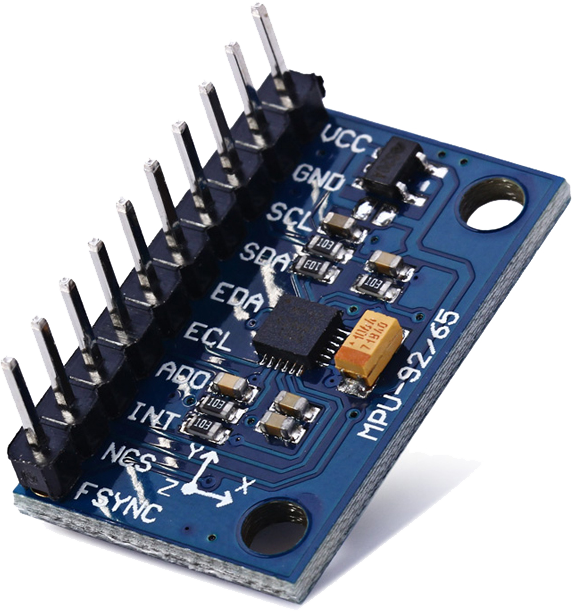
\includegraphics[width=0.5\textwidth]{images/mpu-9250-breakout}
\\MPU-9250 Breakout Board
\end{figure}

\vfill

\begin{flushright}
{\large Heethesh Vhavle \\}
{\large Sanam Shakya \\}
{\large Pushkar Raj \\}
\vspace{0.5cm}
{\large Duration of Internship: $ 22/05/2017-07/07/2017 $ \\}
\end{flushright}
\medskip

{\itshape 2017, e-Yantra Publication}
\end{titlepage}

%-------------------------------------------------------------------------------

%\tableofcontents
%\listoffigures

%-------------------------------------------------------------------------------

\chapter[Sensor Interfacing for Quadcopter]{Sensor Interfacing for Quadcopter}
\section{Introduction}
The project deals with the study of control algorithms and to develop a custom firmware for quadcopter (flight controller) on 32-bit micro-controllers such as the STM32F1xx (ARM® Cortex®-M3 core). The flight controller is designed to control parameters such as the throttle, yaw, pitch and roll and consists of algorithms considering various motion and dynamics. The next step is to analyze the control algorithm to identify effects of various parameters and to optimize it for stable motion. The final step is to develop a wireless joystick controller for simple maneuvering of the quadcopter.\\ 

One of the most trivial and important tasks of a flight controller firmware is control and stabilization of the orientation of the quadcopter. The three axes of orientation involved are namely pitch, roll and yaw as shown in \textit{\autoref{fig:AHRS}}\\

\begin{figure}[!htb]
\centering
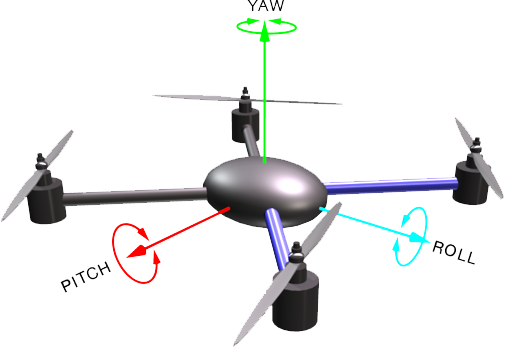
\includegraphics[width=0.6\textwidth]{images/AHRS}
\caption{The pitch, roll and yaw angles (AHRS) of a quadcopter\cite{ardu}}
\label{fig:AHRS}
\end{figure}

\section{Attitude and Heading Reference System}
An \textit{Attitude and Heading Reference System (AHRS)} consists of sensors on three axes that provide attitude information for aircraft, including roll, pitch and yaw. They are designed to replace traditional mechanical gyroscopic flight instruments and provide superior reliability and accuracy.\cite{ahrswiki}\\

AHRS consist of either solid-state or microelectromechanical systems (MEMS) gyroscopes, accelerometers and magnetometers on all three axes. A form of non-linear estimation such as an Extended Kalman filter is typically used to compute the solution from these multiple sources. One abbreviation used in technology for sensor arrays used in AHRS is MARG (Magnetic, Angular Rate, and Gravity).\cite{ahrswiki}\\

\subsection{MPU9250 Accelerometer and Gyroscope}
The \href{./datasheets/MPU9250 Datasheet.pdf}{MPU-9250} is an inertial measurement unit (IMU). MPU-9250 features three 16-bit analog-to-digital converters (ADCs) for digitizing the gyroscope outputs, three 16-bit ADCs for digitizing the accelerometer outputs, and three 16-bit ADCs for digitizing the magnetometer outputs. For precision tracking of both fast and slow motions, the parts feature a user-programmable gyroscope full-scale range of $\pm$250, $\pm$500, $\pm$1000, and $\pm$\SI{42}{\degree\per\second} (dps), a user-programmable accelerometer full-scale range of $\pm$2g, $\pm$4g, $\pm$8g, and $\pm$16g, and a magnetometer full-scale range of $\pm$4800$\mu$T. The MPU-9250 can be interfaced via SPI or I2C. In our case, I2C at \SI{400}{\kilo\hertz} is used to interface the sensor.

\begin{figure}[!htb]
\centering
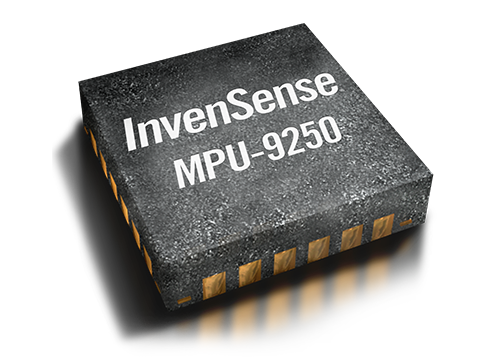
\includegraphics[width=0.4\textwidth]{images/mpu-9250}
\caption{InvenSense MPU-9250 QFN package\cite{mpu9250}}
\end{figure}

\subsubsection{Accelerometer}
Accelerometers are devices that measure static acceleration in all the three axes. Accelerometers are electromechanical devices that sense either static or dynamic forces of acceleration. Static forces include gravity, while dynamic forces can include vibrations and movement. Generally, accelerometers contain capacitive plates internally. Some of these are fixed, while others are attached to miniscule springs that move internally as acceleration forces act upon the sensor. As these plates move in relation to each other, the capacitance between them changes. From these changes in capacitance, the acceleration can be determined. Other accelerometers can be centered around piezoelectric materials. These tiny crystal structures output electrical charge when placed under mechanical stress ( e.g. acceleration).\\

\begin{figure}[!htb]
\centering
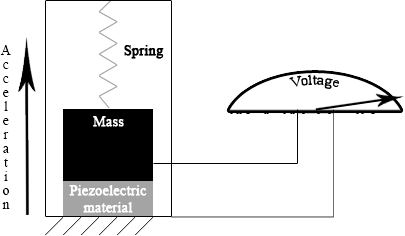
\includegraphics[width=0.6\textwidth]{images/accel_mems}
\caption{An example of the inside of a piezoelectric accelerometer\cite{tonik}}
\label{fig:AHRS}
\end{figure}

They measure in G-forces (g) equivalent to \SI{9.8}{\kilo\gram\meter\per\second\squared}. Most accelerometers will have a selectable range of forces they can measure. These ranges can vary from $\pm$1g up to $\pm$250g. Typically, the smaller the range, the more sensitive the readings will be from the accelerometer. In our case, the selected range is $\pm$4g.\cite{tonik}\\

Assuming no external forces act (except gravity) on the sensor, the pitch and roll angles can easily be computed by knowing the components of gravity in the different axis, which is the sensor output. By using trigonometric formulas, we can easily compute these angles. Practically, the accelerometer not only measures gravity but also all the other vibrations and the output is very noisy. This noise can be filtered out with the help of a gyroscope.\\

\subsubsection{Gyroscope}
The gyroscope sensor within the MEMS is tiny (between 1 to 100 micrometers). When the gyro is rotated, a small resonating mass is shifted as the angular velocity changes. This movement is converted into very low-current electrical signals that can be amplified and read by a host micro-controller \cite{gyro}. The range of the gyroscope selected is $\pm$1000 dps.\\

\begin{figure}[!htb]
\centering
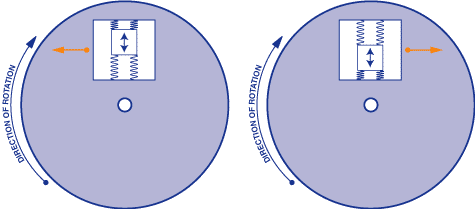
\includegraphics[width=0.7\textwidth]{images/gyro_mems}
\caption{Internal operational view of a MEMS gyro sensor\cite{gyro}}
\end{figure}

However, the gyroscope output doesn't give the angular orientation. It gives the angular rate of orientation around the three axes. This rate has to be integrated over time in order to obtain the orientation angles. But the main disadvantage of the gyroscope is that its value drifts over time due to rounding off errors and keeps accumulating these errors as we integrate it.\\

One of the solutions to combat this problem is to fuse the sensor data from both the accelerometer and the gyroscope. A simple filter like a complimentary filter can be used to achieve this. The result of this filter is pretty good. The accelerometer provides gravity as an absolute reference and helps to correct the drift from of the gyroscope.\\ 

However, this solution only provides us with only the pitch and roll angles. We also require to know the heading of the quadcopter or the yaw angle. Although, the gyroscope can measure the yaw rate of rotation, the accelerometer has no means to detect a change in yaw direction, as it only refers to gravity. Without a reference in the yaw direction, the gyroscope output will again drift. Now, that's where the Magnetometer comes in to provide this absolute reference.\\

\clearpage

\subsubsection{Sensor Initialization}
Following is a snippet explaining the initialization of the IMU. It is always a safe practice to verify the device ID of the sensor, so that we know the I2C interface is successful and if not, handle the error. The register names are macros defined in the \textit{MPU9250.h} header file. Address values and register bits are explained in detail in the \href{./datasheets/MPU9250 Register Map.pdf}{MPU-9250 Register Map}.\\  

\begin{minted}[linenos=true]{c}
// Verify device by comparing the WHO_AM_I register value
uint8_t data = I2C_ReadByte(MPU9250_ADDRESS, WHO_AM_I, __FILE__, __LINE__);
 
// Device verification failed 
if (data != WHO_AM_I_VALUE) _Error_Handler(__FILE__, __LINE__);
\end{minted}

\bigskip
The next step is to first reset the device, enable the sensors and configure the internal clock source. Settings such as digital low pass filtering and full scale range can be configured as shown below.\\

\begin{minted}[linenos=true]{c}
// Reset
I2C_WriteByte(MPU9250_ADDRESS, MPU_PWR_MGMT_1, 0x80, 1);
 
// Set clock source to be PLL
I2C_WriteByte(MPU9250_ADDRESS, MPU_PWR_MGMT_1, 0x01, 1); 
 
// Enable Accel and Gyro
I2C_WriteByte(MPU9250_ADDRESS, MPU_PWR_MGMT_2, 0x00, 1); 
 
// Sample Rate Divider (Not set) 
I2C_WriteByte(MPU9250_ADDRESS, SMPLRT_DIV, 0x00, 1); 
 
// DLPF 184Hz 
I2C_WriteByte(MPU9250_ADDRESS, ACCEL_CONFIG2, 0x03, 1); 
I2C_WriteByte(MPU9250_ADDRESS, MPU9250_CONFIG, 0x03, 1);

// Full scale settings
I2C_WriteByte(MPU9250_ADDRESS, GYRO_CONFIG, GYRO_FS_1000_DPS, 1);
I2C_WriteByte(MPU9250_ADDRESS, ACCEL_CONFIG, ACC_FS_4_G, 1);
\end{minted}

\clearpage

\subsubsection{Reading the Sensor Data}
The initialization function will have to be called once and after that the raw data from the sensors can be read, converted and compensated at fixed refresh rate. The chosen refresh rate must be less than the update rate of the sensor. MPU-9250 has an update rate of \SI{1}{\kilo\hertz}. The raw data is available in the output registers in series, starting with the X axis. The output of each axis is a 16-bit value and is available as set of two bytes (high and low). Therefore, six bytes of data will have to be read in series (two for each axis) and they must be packed back to a 16-bit value.\\

\begin{minted}[linenos=true]{c}
// Data buffer to store the raw data
uint8_t raw_data[] = {0, 0, 0, 0, 0, 0};

// Read raw data
I2C_ReadByteArray(MPU9250_ADDRESS, ACCEL_XOUT_H, raw_data, 6);

// Pack it to 16-bits and store it
accelRaw.x = (int16_t) ((raw_data[0]<<8) | raw_data[1]);
accelRaw.y = (int16_t) ((raw_data[2]<<8) | raw_data[3]);
accelRaw.z = (int16_t) ((raw_data[4]<<8) | raw_data[5]);
\end{minted}

\bigskip
The raw data is just a numerical value ranging from -32768 to +32767. This data will have to be converted to G-units. The conversion depends on the full scale range settings chosen for the sensor. Here the setting chosen was $\pm4$ and the conversion is performed as follows.\\

\begin{minted}[linenos=true]{c}
accelData.x = (float) accelRaw.x * 4.0f/32768.0f;
accelData.y = (float) accelRaw.y * 4.0f/32768.0f;
accelData.z = (float) accelRaw.z * 4.0f/32768.0f;
\end{minted}

\bigskip
Similarly, the gyroscope data can be obtained, the only difference being the conversion factor. When the sensor is kept in static position, the output of the gyroscope will still be non-zero. This gyroscope bias can calculated by taking multiple samples when kept still, and then averaging it.\\

\begin{minted}[linenos=true]{c}
gyroData.x = ((float) gyroRaw.x * 1000.0f/32768.0f) - gyroBias.x;
gyroData.y = ((float) gyroRaw.y * 1000.0f/32768.0f) - gyroBias.y;
gyroData.z = ((float) gyroRaw.z * 1000.0f/32768.0f) - gyroBias.z;
\end{minted}

\clearpage

\subsection{AK8963 Magnetometer}
\label{ssec:akmag}
The AK8963 Magnetometer is 3-axis electronic compass IC with high sensitive Hall sensor technology. This sensor is interfaced as an auxiliary sensor to the MPU-9250. The MPU-9250 acts as a master to any external sensors connected to the auxiliary I2C bus. To access the magnetometer via MPU-9250, the \textit{BYPAS{\_}EN} bit in the \textit{INT Pin / Bypass Enable Configuration} register of the MPU-9250 has to be set. Further details about this can be found in  \href[page=23]{./datasheets/MPU9250 Datasheet.pdf}{Page 23 - Datasheet}. The initialization snippet is shown below.\\

\begin{minted}[linenos=true]{c}
/* Enable access to Magnetometer via MPU-9250 */
// Set bypass mode for external I2C master connection
I2C_WriteByte(MPU9250_ADDRESS, INT_PIN_CFG, 0x22, 1);	

// Verify magnetometer device ID
uint8_t data = I2C_ReadByte(MAG_ADDRESS, MAG_WIA);
if (data != MAG_WIA_VALUE) _Error_Handler(__FILE__, __LINE__);

// Reset magnetometer
I2C_WriteByte(MAG_ADDRESS, MAG_CNTL2, 0x01, 1);
\end{minted}

\bigskip

\subsubsection{Magnetometer Biases}
Magnetometers are wonderful devices and absolutely essential for correcting gyro drift in applications that require absolute orientation through sensor fusion. The bane of magnetometer usage is, however, their non-ideal response surfaces. The ideal response surface for a three-axis magnetometer is a sphere centered at the 3D origin. This means the response to an external magnetic field of, let's say 400 milliGauss (mG) in the z-direction would be exactly Mz = 400 mG when the magnetometers z-axis was normal to the floor, My = 400 mG when the magnetometer's y-axis was normal to the floor, and Mx = 400 mG when the magnetometer's x-axis was normal to the floor. More simply, the ideal response surface no matter the orientation of the magnetometer is a sphere with radius 400 mG centered on the origin. In practice, MEMS magnetometers are rarely so well calibrated when you receive them. There are good reasons for this. The MEMS sensors are typically characterized at the factory but mounting on a PC board can add stresses that can easily result in a shift of the calibration.\cite{kris}\\

\clearpage

\subsubsection{Sensor Initialization}
The first set of calibration process is to compensate the raw data with the help of factory calibrated data. The factory sensitivity adjustment data for each axis is stored in fuse ROM on shipment. These scaling factors can be read from the ROM as follows.\\

\begin{minted}[linenos=true]{c}
// Power down magnetometer		
I2C_WriteByte(MAG_ADDRESS, MAG_CNTL1, 0x00, 1);	

// Enter Fuse ROM access mode	
I2C_WriteByte(MAG_ADDRESS, MAG_CNTL1, 0x0F, 1); 	

// Read calibration registers for sensitivity adjustment values
uint8_t rawData[3];
I2C_ReadByteArray(MAG_ADDRESS, MAG_ASAX, rawData, 3);

// Calculate and store the adjusted measurement data
magCalib.x =  (float)(rawData[0] - 128)/256.0f + 1.0f;   
magCalib.y =  (float)(rawData[1] - 128)/256.0f + 1.0f;
magCalib.z =  (float)(rawData[2] - 128)/256.0f + 1.0f;
\end{minted}

\bigskip

AK8963 has seven \href[page=13]{./datasheets/AK8963.pdf}{operation modes}. \href[page=15]{./datasheets/AK8963.pdf}{Continuous measurement mode 2} is used in our case. Sensor is measured periodically in 100Hz in this mode and the configuration snippet is shown below.\\

\begin{minted}[linenos=true]{c}
// Power down magnetometer
I2C_WriteByte(MAG_ADDRESS, MAG_CNTL1, 0x00, 1);

// Res: 16 Bit, Mode: Continuous Mode 2 (100Hz)		
I2C_WriteByte(MAG_ADDRESS, MAG_CNTL1, 0x16, 1); 
\end{minted}

\bigskip
\bigskip

In spite of the factory calibration, the problem of non-ideal response of the sensor in various axes, which was mentioned earlier, still persists. The data plotted in \textit{\autoref{fig:magraw}} was taken by slowly turning the sensor board through a variety of figure-eight patterns. The data is properly-scaled (mG) Mx, My, and Mz values plotted using \textit{Matplotlib} in Python. Following are the observations that can be inferred from the uncalibrated sensor data.\\

\bigskip

\begin{figure}[!htb]
\centering
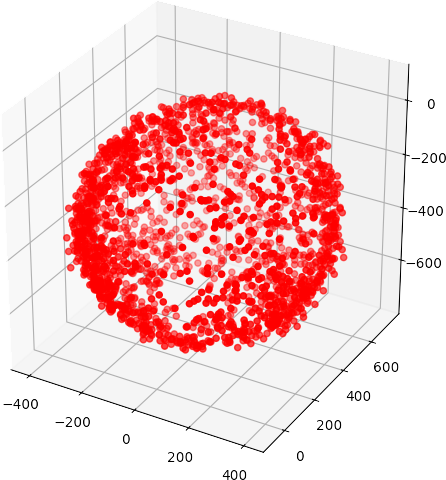
\includegraphics[width=0.7\textwidth]{images/raw}
\caption{Magnetic field in mG along X, Y and Z axes measured for an uncalibrated sensor}
\label{fig:magraw}
\end{figure}

\begin{enumerate}
\item The response between axes is not centered at the origin.
\item The response sensitivity is different along each axis. 
\end{enumerate}

These are often referred to as hard iron and soft iron biases, respectively. Calculating these biases is explained in \textit{Section \ref{sssec:mag_calib}}. \\

\textbf{Hard iron biases} are typically the largest and the easiest errors to correct for. The simplest way to correct for them is to record a bunch of magnetometer data as the sensor is moved slowly in a figure eight pattern and keep track of the minimum and maximum field measured in each of the six principal directions; +/- Mx, +/- My, +/- Mz. Once the min/max values along the three axes are known, the average can be subtracted from the subsequent data which amounts to re-centering the response surface on the origin \cite{kris}. \textit{\autoref{fig:magoffset}} shows the hard iron bias calibrated sensor data.\\

\begin{figure}[!htb]
\centering
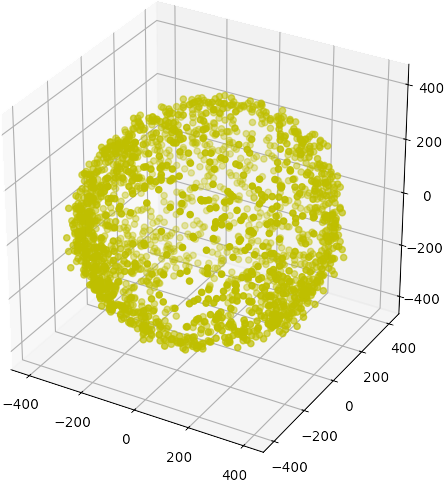
\includegraphics[width=0.57\textwidth]{images/offset}
\caption{The AK8963 magnetometer data after subtraction of the three axial offset biases}
\label{fig:magoffset}
\end{figure}

\begin{figure}[!htb]
\centering
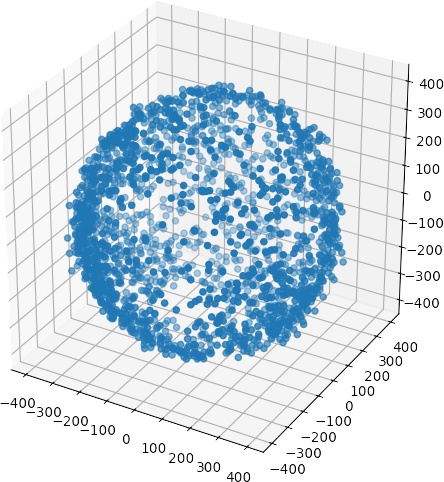
\includegraphics[width=0.57\textwidth]{images/scaled}
\caption{The MPU9250 magnetometer response after offset and scaling bias corrections}
\label{fig:magscale}
\end{figure}

\clearpage
\textbf{Soft iron bias} correction is re-scaling the axial response to make is even more spherical. It means deconstructing the response surface into its elliptical principle axes and devising a 3 x 3 correction matrix to transform the general ellipsoidal response surface into a spherical one. The min/max values which are already computed are used to rescale the magnetometer data and compute a scale factor for all three axes. Finally, the calibrated sensor data is shown in \textit{\autoref{fig:magscale}}.\cite{kris}\\

\subsubsection{Reading the Sensor Data}
Once all of the initialization and calibration is performed, the data can be read from the sensor now. There are certain points to note before we can read the data. When measurement data is stored and ready to be read, DRDY (Data Ready) bit in ST1 register turns to \textit{“1”} and this condition has to be checked first \textit{(line 2)}.\\

AK8963 has the limitation for measurement range that the sum of absolute values of each axis should be smaller than 4912$\mu$T.

\begin{center}
$\mid X \mid + \mid Y \mid + \mid Z \mid  <  4912 \mu T$
\end{center}

When the magnetic field exceeds this limitation, data stored at measurement data is not correct. This is called Magnetic Sensor Overflow. When magnetic sensor overflow occurs, HOFL bit in ST2 register turns to \textit{“1”}. When the next measurement starts, it returns to \textit{“0”} \textit{(line 9)}. Also it is necessary that a read operation on the ST2 register has to be performed in order to initiate the next conversion cycle \textit{(line 5)}.\\ 

Another thing to note is, unlike the MPU-9250, the raw data here is available as low byte first, then the high byte. Once the raw data has packed into 16-bit the factory calibration is applied. Now, the raw data has to be converted to milliGauss and \textit{mRes} is the conversion factor.

\begin{center}
$ mRes = 10.0 \times 4912.0/32760.0$
\end{center}

\bigskip

The final step is to compensate the converted data with the hard and soft iron biases. Calculating these biases is explained in \textit{Section \ref{sssec:mag_calib}}.\\ 

\begin{minted}[linenos=true]{c}
// Check if data is ready
if (I2C_ReadByte(MAG_ADDRESS, MAG_ST1, __FILE__, __LINE__) & 0x01)
{
  // Read data registers and ST2 register to check overflow
  I2C_ReadByteArray(MAG_ADDRESS, MAG_HXL, raw_data, 7, __FILE__, __LINE__);
  uint8_t OVF = raw_data[6];

  // Store data if no overflow occurred
  if (!(OVF & 0x08))
  {
    // Pack into 16-bit data
    magRaw.x = (int16_t) ((raw_data[1]<<8) | raw_data[0]);
    magRaw.y = (int16_t) ((raw_data[3]<<8) | raw_data[2]);
    magRaw.z = (int16_t) ((raw_data[5]<<8) | raw_data[4]);

    // Apply the factory calibration and conversion factors
    magData.x = (float) magRaw.x * mRes * magCalib.x; 
    magData.y = (float) magRaw.y * mRes * magCalib.y; 
    magData.z = (float) magRaw.z * mRes * magCalib.z; 
    
    // Apply the hard iron and soft iron bias corrections
    magData.x = (magData.x - magBias.x) * magScale.x;
    magData.y = (magData.y - magBias.y) * magScale.y;
    magData.z = (magData.z - magBias.z) * magScale.z;
}
\end{minted}

\subsubsection{Magnetometer Calibration}
\label{sssec:mag_calib}

Currently, the hard and soft iron bias calibration is not implemented in the firmware and has to performed externally. To do this, the converted magnetometer readings are just printed on the serial terminal and then stored as \textit{*.csv} file. The calibration is done using a Python script. The \textit{*.csv} file of uncalibrated readings are read and the following steps are carried out in order to get the bias values.\\

\begin{enumerate}
\item Find out the maximum and the minimum values for each of the axes from the data samples.\\
\item Find the average of the maximum and the minimum values.\\
\item This average value is nothing but the hard iron bias value.\\
\item To find out the soft iron bias, calculate the range of the data samples. This is just the difference between the maximum and minimum value.\\
\item Find out the average of the range of all the three axes.\\
\item The average value divided by the range of each axis gives the scaling factor for that respective axis. This is the soft iron bias.\\
\end{enumerate}

Following is a snippet from the \textit{mag-calib.py} Python script, implementating the calibration process.\\

\begin{minted}[linenos=true]{python}
# max_ and min_ are lists which store the maximum and minimum 
# values for the three axes, from the data samples
for i in range(0,3):
    # Find the hard iron bias
    bias[i] = (max_[i] + min_[i])/2
    
    # Find the range to calculate soft iron bias
    range_[i] = max_[i] - min_[i]

# Average of the range of three axes
avg = (range_[0] + range_[1] + range_[2])/3

# Calculate the scaling factor or the soft iron bias for each axis
for i in range(0,3):
    scale[i] = avg/range_[i]
\end{minted}

\bigskip

There is an additional common type of magnetometer bias often encountered which is due to the presence of man-made sources of magnetic field like big steel buildings and current carrying wires, etc. Encounters with these environmental sources of magnetic field can be interpreted as changes in orientation if a magnetic anomaly algorithm is not employed to detect and prevent it. This is beyond the scope of the project right now and can be dealt with in future developement of the firmware. \cite{kris}

\subsection{Sensor Fusion using Madgwick's AHRS Filter}
A MARG (Magnetic, Angular Rate, and Gravity) sensor is a hybrid IMU which incorporates a tri-axis magnetometer. An IMU alone can only measure an attitude (pitch and roll angles) relative to the direction of gravity which is sufficient for many applications. MARG systems, also known as AHRS (Attitude and Heading Reference Systems) are able to provide a complete measurement of orientation relative to the direction of gravity and the earth's magnetic field.\cite{madgwick}\\

The task of an orientation filter is to compute a single estimate of orientation through the optimal fusion of gyroscope, accelerometer and magnetometer measurements. The Kalman filter has become the accepted basis for the majority of orientation filter algorithms. However, implementation of these filters demand a large computational load and not very efficient for embedded systems.\cite{madgwick}\\

Madgwick's algorithm uses a quaternion representation, allowing accelerometer and magnetometer data to be used in an analytically derived and optimised gradient descent algorithm to compute the direction of the gyroscope measurement error as a quaternion derivative. The library for Madgwick's AHRS filter is available \href{http://x-io.co.uk/open-source-imu-and-ahrs-algorithms/}{here} and further details of the working of the filter can be found \href{./datasheets/Madgwick Internal Report.pdf}{here}.\cite{madgwick}\\

Following is a snippet which shows how to use the AHRS filter. Notice the change in sign and axis while passing the IMU data to the filter. \textit{AHRS{\_}Angle} is a float array to store the filtered angles.\\

\begin{minted}[linenos=true]{c}
// Set integration time by time elapsed since last filter update
AHRS_timeNow = millis();
float delta = (float)((AHRS_timeNow - AHRS_lastUpdate)/1000.0f) ;
MadgwickSetDelta(delta);
AHRS_lastUpdate = AHRS_timeNow;

// Filter data and obtain the angles
MadgwickQuaternionUpdate(-accelData.y, -accelData.x, accelData.z, 
	gyroData.y, gyroData.x, -gyroData.z, magData.x, magData.y, 
	magData.z, AHRS_Angle);
\end{minted}

\clearpage

\section{Altitude Measurement}
Altitude can be determined based on the measurement of atmospheric pressure. The greater the altitude, the lower the pressure. When a barometer is supplied with a nonlinear calibration so as to indicate altitude, the instrument is called a pressure altimeter or barometric altimeter. It is very important to know the altitude of a flight and altitude stabilization is required for better control of the quadcopter.

\subsection{MS5611 Barometer}
The MS5611 is a barometric pressure sensor is optimized for altimeters and variometers with an altitude resolution of 10 cm. This sensor is also interfaced on the same I2C bus as that of the IMU.\\

In order to estimate the altitude, first we have to get the pressure  and temperature data from the sensor. The pressure and temperature data is obtained as 24-bit word (3 bytes) after internal ADC conversion. However, this data may not be very useful and must be calibrated and compensated before using them. The MS5611 has a 128 bit PROM where six calibration co-efficients are stored permanently. Using these co-efficients (can be read and stored on the STM32 ROM once initially), the temperature and temperature compensated pressure can be calculated. The compensation and data conversion procedure is explained in the \href[page=7]{./datasheets/MS5611-01BA03.pdf}{datasheet}.\\

Now that we have the current pressure (in millibar), by knowing the pressure at sea level (1013.25 millibar), the altitude can be estimated by using the following formula.\\

\begin{minipage}{\textwidth}
\centering
$Altitude = 44330 \times \left [1 - \left (\frac{P}{P_{0}}\right )^{\frac{1}{5.255}} \right ]$
\end{minipage}
\clearpage

\begin{thebibliography}{20}
%\addcontentsline{toc}{chapter}{References}

\bibitem{ahrswiki}
Wikipedia Article, \href{https://en.wikipedia.org/wiki/Attitude_and_heading_reference_system}{\textit{Attitude and heading reference system}}

\bibitem{ardu}
Arducopter, \href{http://www.arducopter.co.uk/all-arducopter-guides/arducopter-flight-modes}{\textit{
Arducopter Flight Modes}}, 2013

\bibitem{mpu9250}
InvenSense, \href{https://www.invensense.com/products/motion-tracking/9-axis/mpu-9250/}{\textit{MPU-9250 Nine-Axis (Gyro + Accelerometer + Compass) MEMS MotionTracking™ Device}}

\bibitem{tonik}
Toni Corinne, \href{https://learn.sparkfun.com/tutorials/accelerometer-basics}{\textit{Accelerometer Basics}} at SparkFun

\bibitem{gyro}
A1ronzo, \href{https://learn.sparkfun.com/tutorials/gyroscope/how-a-gyro-works}{\textit{Gyroscope}} at SparkFun

\bibitem{kris}
Kris Winer, \href{https://github.com/kriswiner/MPU6050/wiki/Simple-and-Effective-Magnetometer-Calibration}{\textit{Simple and Effective Magnetometer Calibration}}

\bibitem{madgwick}
Sebastian O.H. Madgwick, \href{./datasheets/Madgwick Internal Report.pdf}{\textit{An efficient orientation filter for inertial and inertial/magnetic sensor arrays}}

\end{thebibliography}

%-------------------------------------------------------------------

\end{document}

